%%%%%%%%%%%%%%%%%%%%%%%%%%%%%%%%%%%%%%%%%%%%%%%%%%%%%%%%%%
%% LAYOUT PARA A DISSERTAÇÃO NA UNIVERSIDADE DA MADEIRA %%
%% Implementado por Ivan Teixeira (Zlynt)               %%
%%%%%%%%%%%%%%%%%%%%%%%%%%%%%%%%%%%%%%%%%%%%%%%%%%%%%%%%%%

\documentclass[12pt]{article}
\usepackage{graphicx}
\usepackage{tikz}
\usepackage{fontspec}
\definecolor{verde_titulo}{RGB}{143, 207, 44}
\definecolor{cor_autor}{RGB}{87,87,99}
\definecolor{cor_curso}{RGB}{147,147,151}
\definecolor{cor_ano}{RGB}{36,145,173}

\newcommand{\smalltonormalsize}{%
  \fontsize
    {\fpeval{(\f@size@small+\f@size@normalsize)/2}}
    {\fpeval{(\f@baselineskip@small+\f@baselineskip@normalsize)/2}}%
  \selectfont
}
\usepackage[left=-0.65cm,top=0cm,right=0cm,bottom=0cm,verbose,nohead,nofoot]{geometry}


\usepackage[utf8]{inputenc}
\setmainfont{Arial}


%\title{[UMa] Layout Tese}
%\author{ivan.goncalo }
%\date{November 2020}


\begin{document}

% Capa da Tese
\pagenumbering{gobble}

%\textcolor{blue}{\MakeUppercase{Título da Dissertação}}

\begin{tikzpicture}

\node[inner sep=0pt] at (current page.center) (X) {
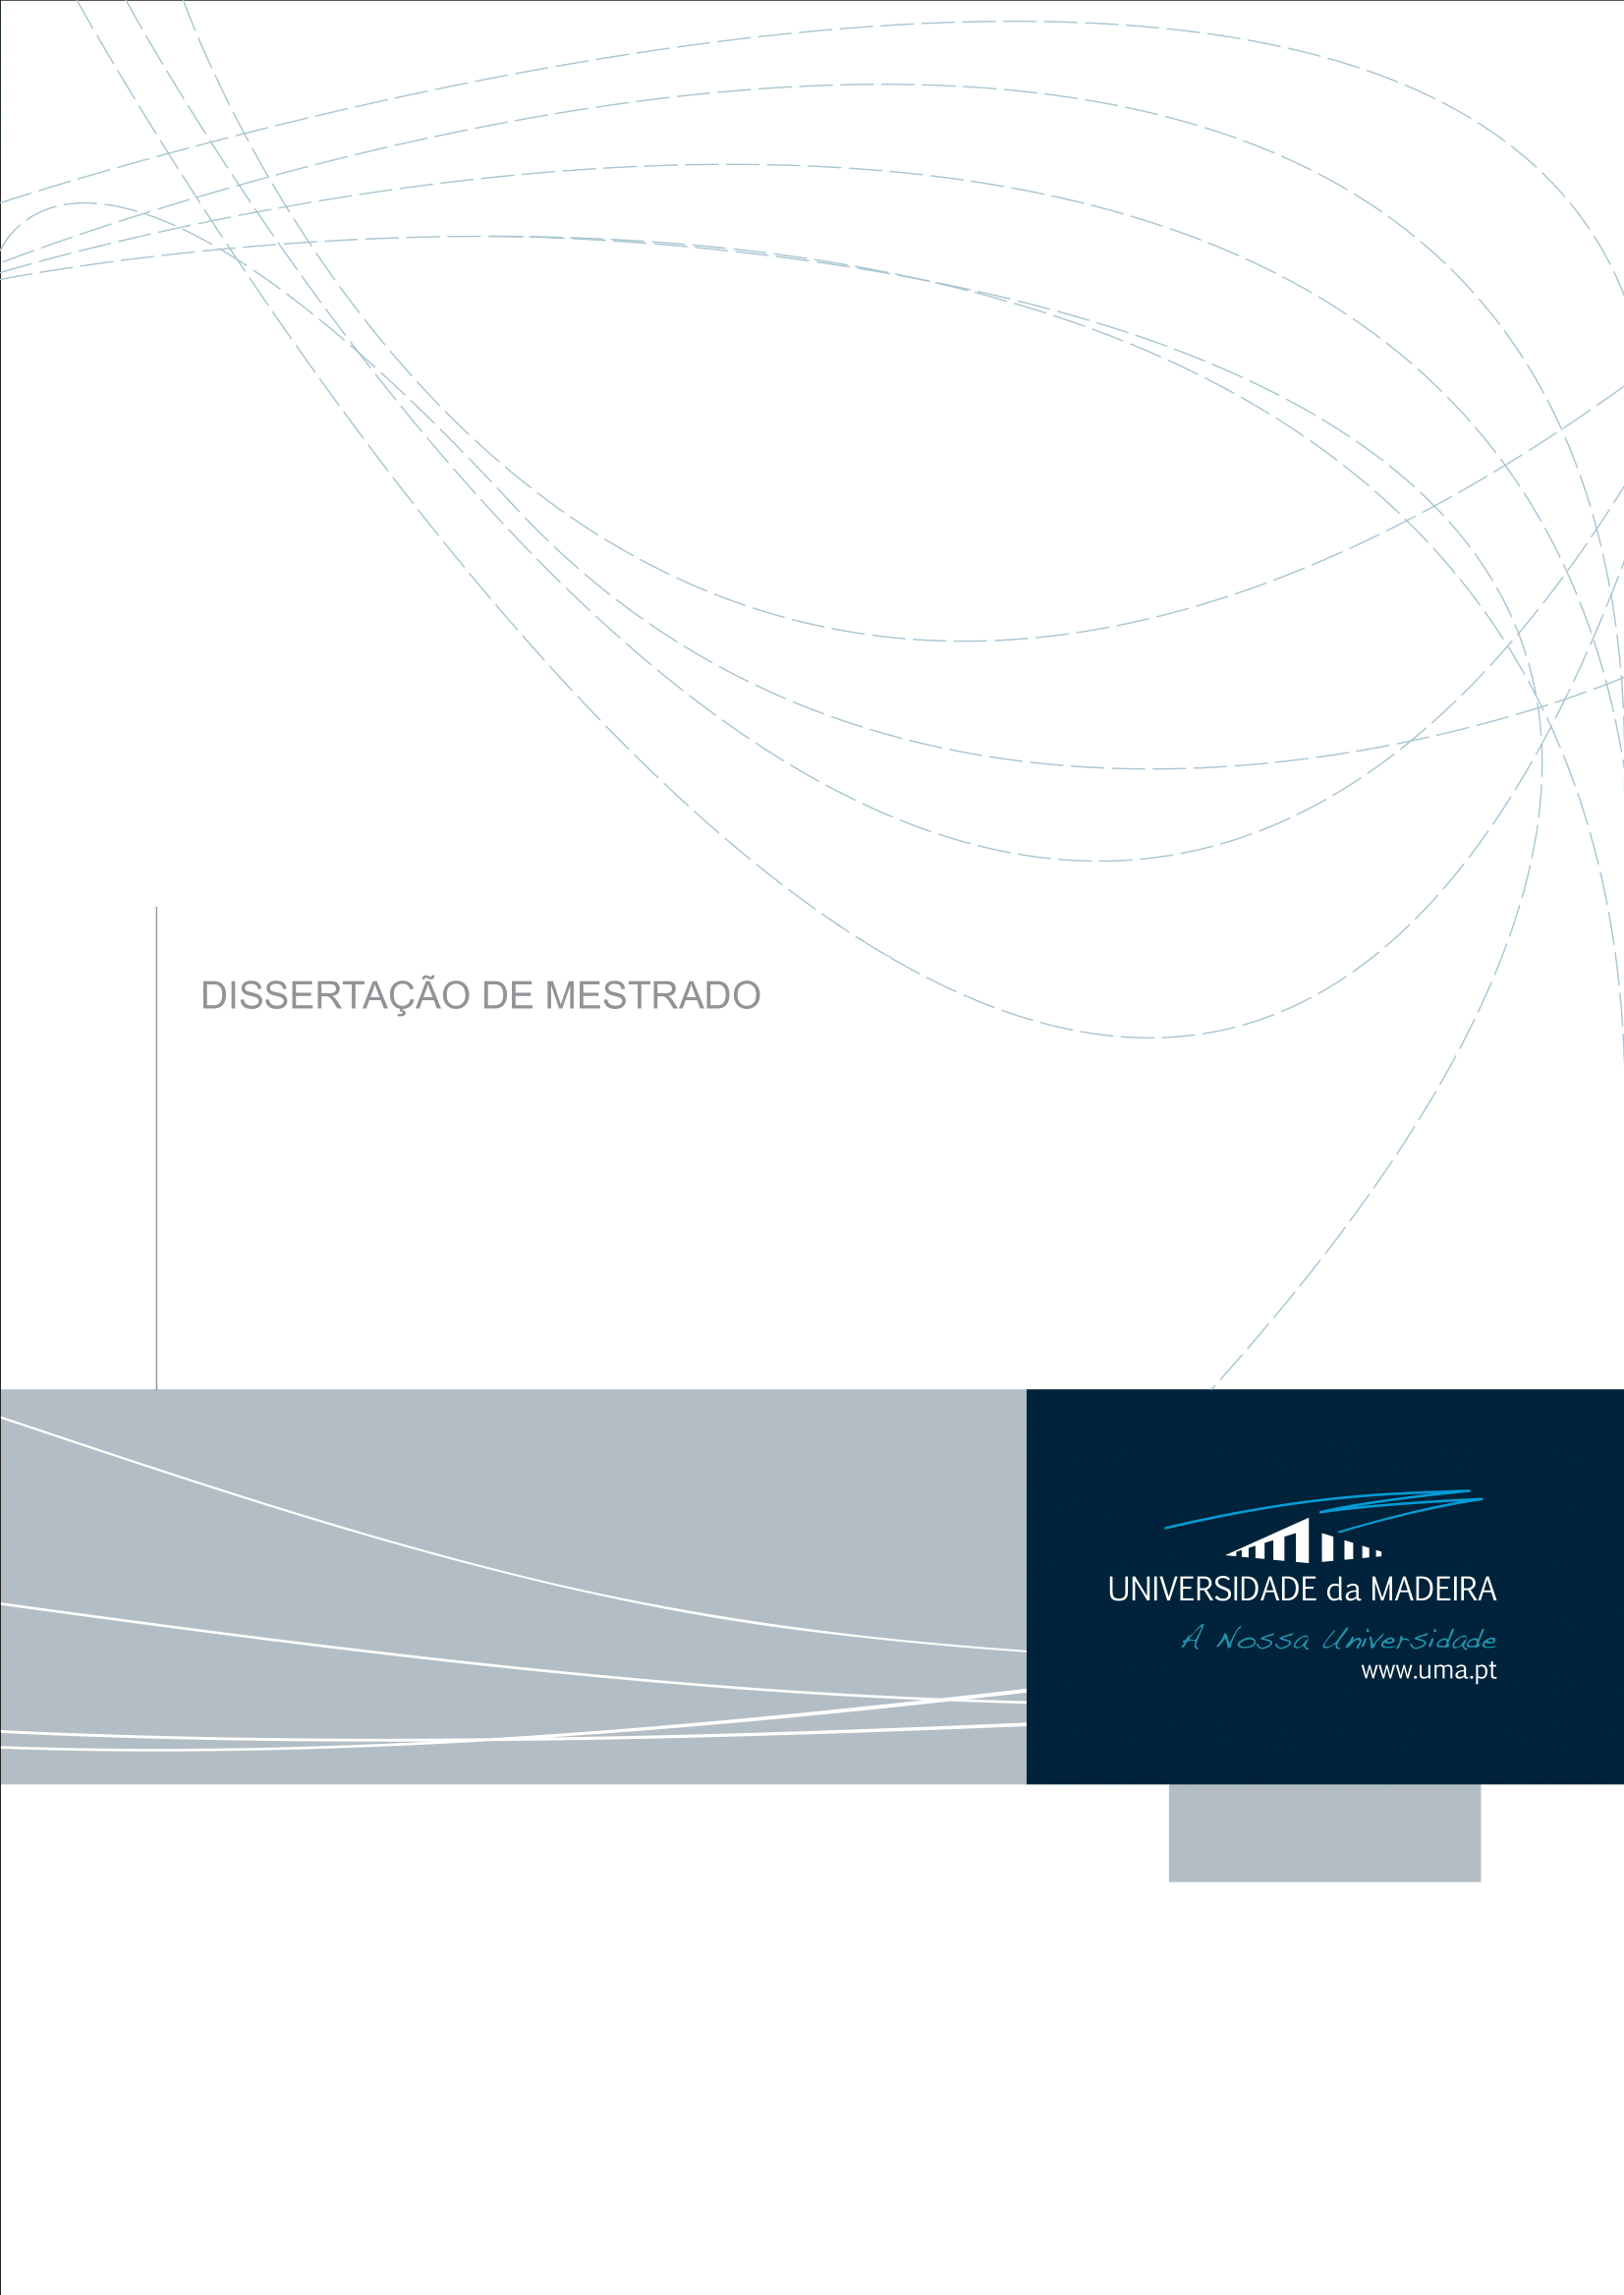
\includegraphics[width=\paperwidth,height=0.9\paperheight]{Imagens/Fundo1.png}
};

\begin{scope}[x={(X.south east)},y={(X.north west)}]
\fill[fill = white,fill opacity=0.6] ($(X.south west) + (0,1in)$) rectangle ($(X.north east) - (0,1in)$);

%Titulo da Dissertação
\node[text width=10in] (Z) at (0.70,0.5735) {
\addfontfeature{LetterSpace=11.0}

   \fontsize{17.5pt}{17.5pt}\textcolor{verde_titulo}{\MakeUppercase{\spaceskip=1.8\fontdimen3\textbf{
   Título da Dissertação
   }}}
};

%Nome do Autor
\node[text width=10in] (Z) at (0.704,0.4625) {
\addfontfeature{LetterSpace=11.0}

   \fontsize{13pt}{13pt}\textcolor{cor_autor}{\spaceskip=1.8\fontdimen3\textbf{
   Nome do Autor
   }}
};

%Curso do Mestrado
\node[text width=10in] (Z) at (0.706,0.446) {
\addfontfeature{LetterSpace=3.0}

   \smalltonormalsize\textcolor{cor_curso}{\spaceskip=1.8\fontdimen3\MakeUppercase{
   Mestrado em ...
   }}
};

%Mês
\node[text width=10in] (Z) at (1.332,0.177) {
\addfontfeature{LetterSpace=12.0}

   \smalltonormalsize{\spaceskip=1.8\fontdimen3
   \textbf{\textcolor{white}{
   Fevereiro
   } \textcolor{cor_ano}{
   | 2010
   }}
   }
};


\end{scope}%
%Tamanho do texto: 0.705cm
%\node [below left,align=center] at (imagem_fundo.center){
%\textcolor{verde_titulo}{\MakeUppercase{\textbf{Título da Dissertação}}}
%};




\end{tikzpicture}



%\tikz[remember picture,overlay] \node[opacity=0.5,inner sep=0pt] at (current page.center){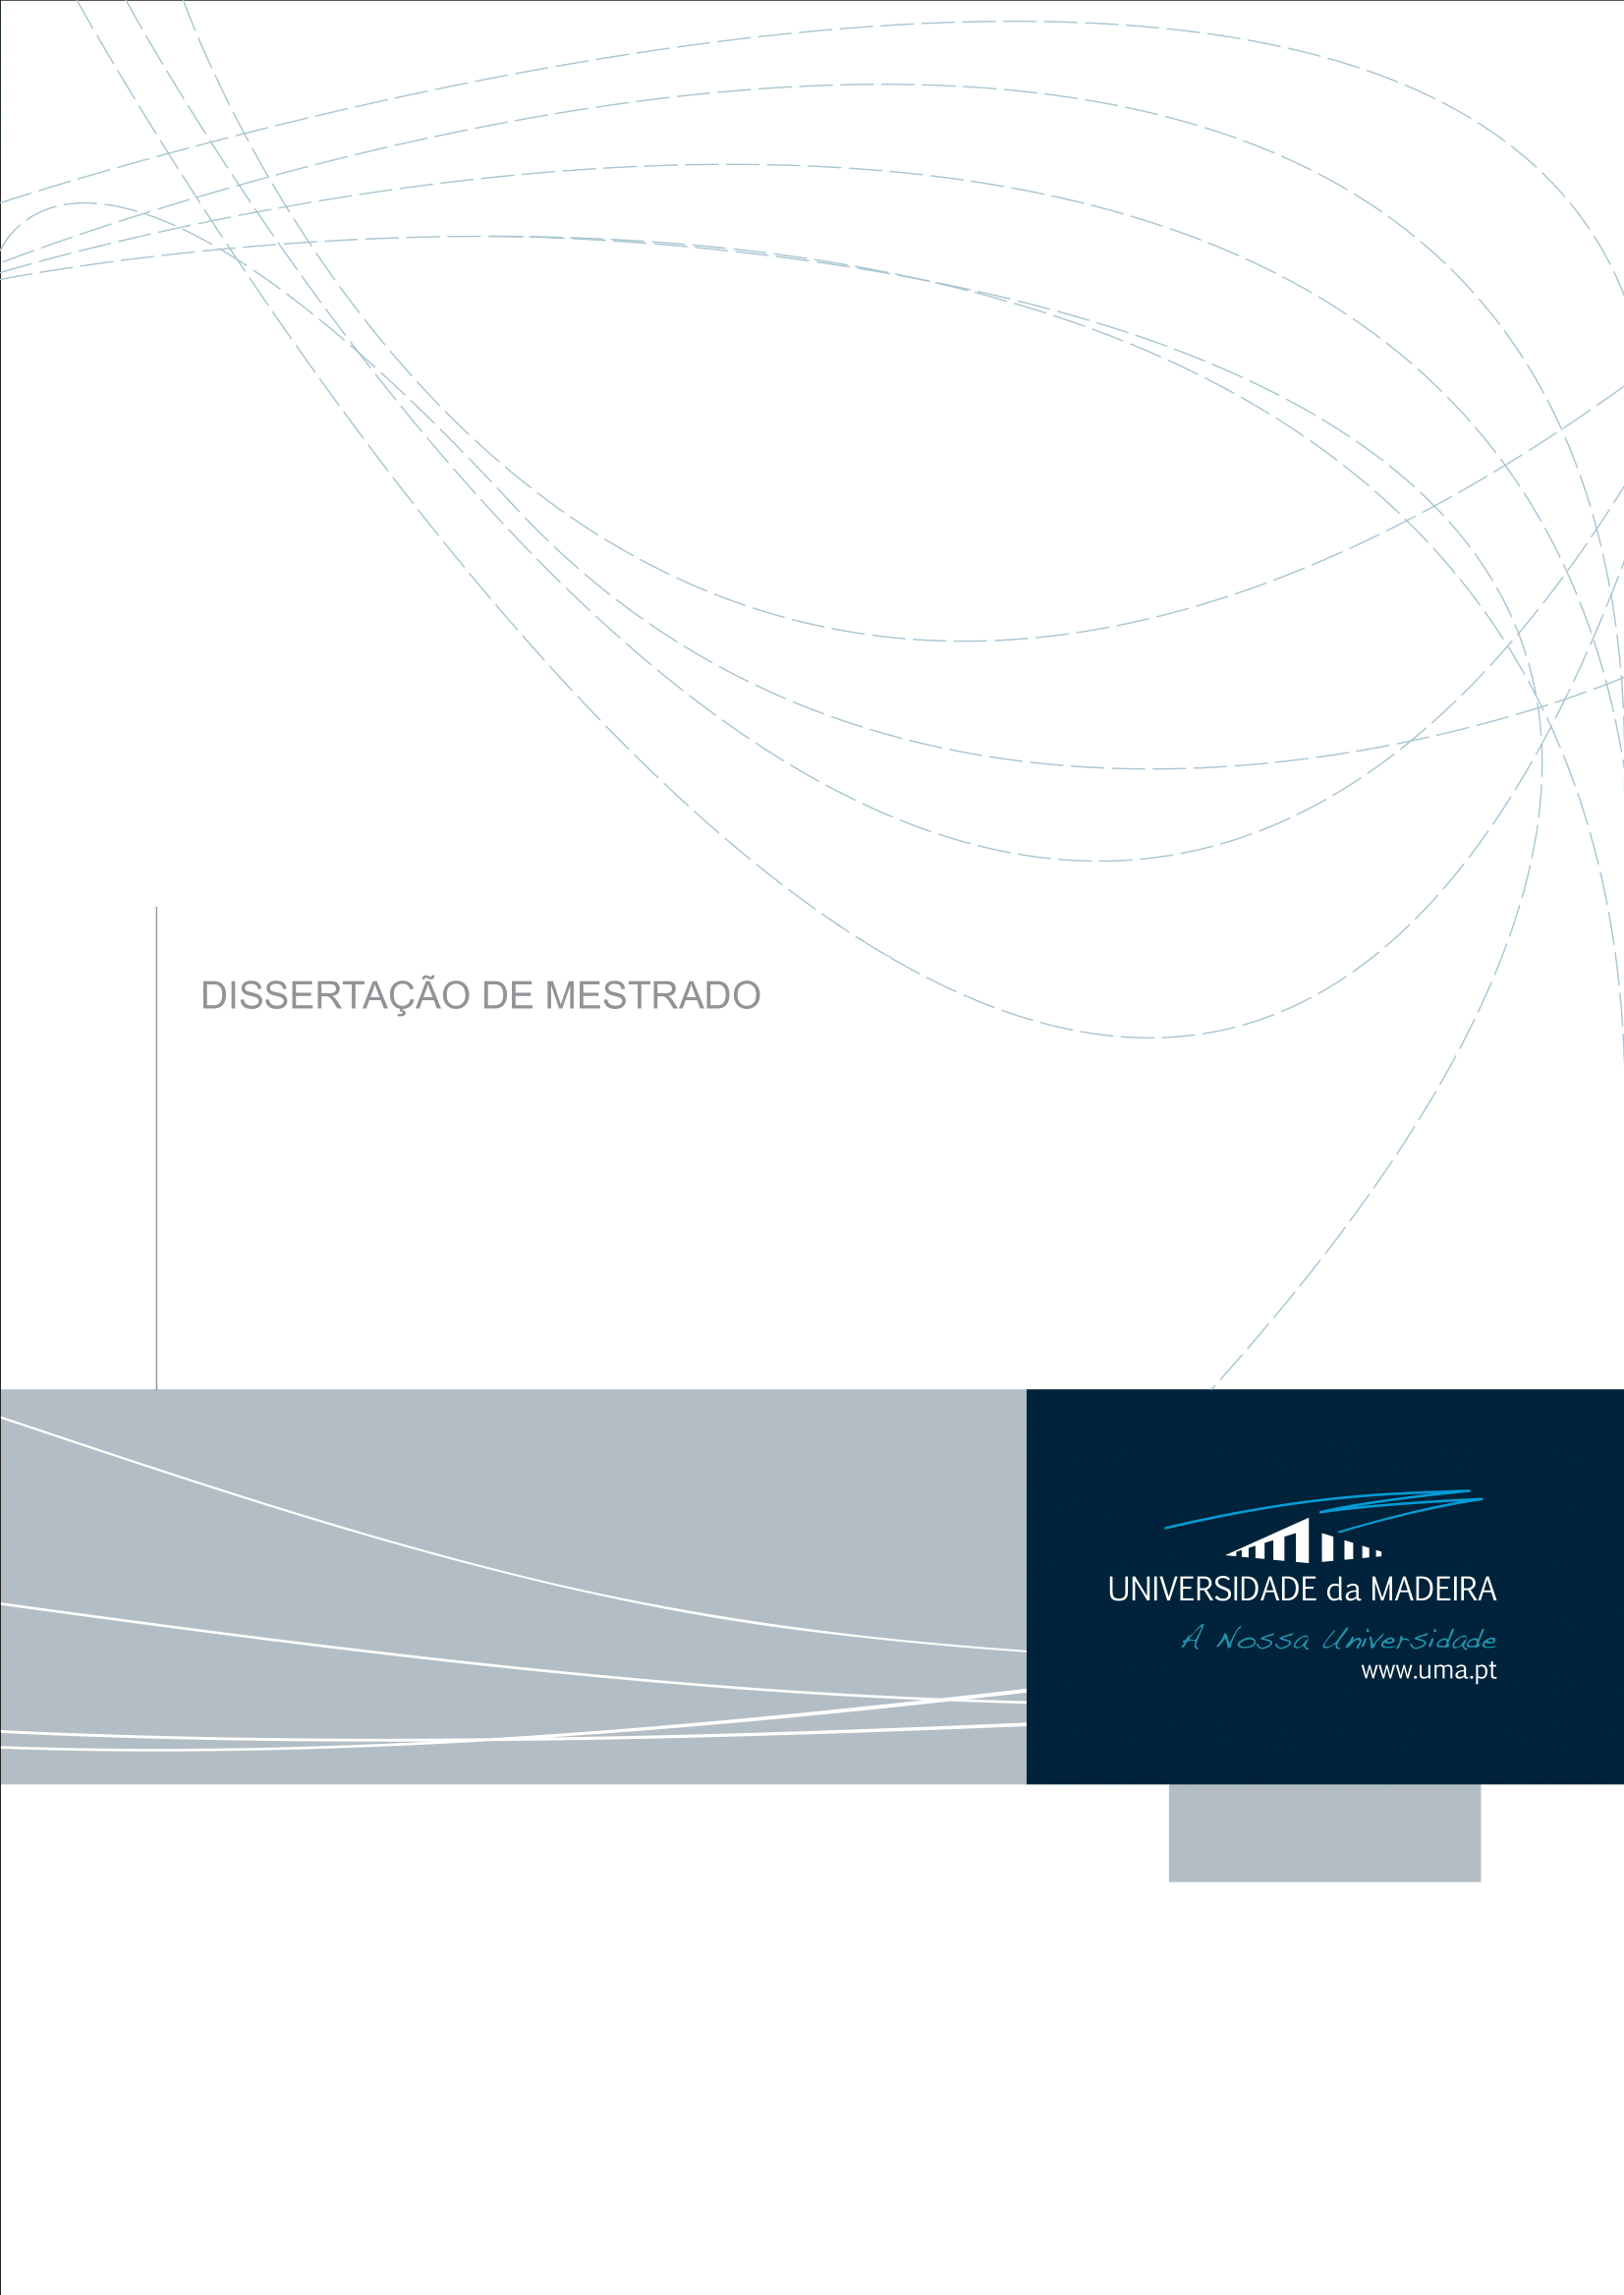
\includegraphics[width=\paperwidth,height=\paperheight]{Imagens/Fundo1.png}};

\restoregeometry
\clearpage



%\maketitle
Hello World From Thesis

%\section{Introduction}

\end{document}
